\documentclass[a4paper,14pt]{article} % тип документа
%\documentclass[14pt]{extreport}
\usepackage{extsizes} % Возможность сделать 14-й шрифт


\usepackage{geometry} % Простой способ задавать поля
\geometry{top=20mm}
\geometry{bottom=25mm}
\geometry{left=15mm}
\geometry{right=15mm}

\setcounter{section}{0}

%%%Библиотеки
%\usepackage[warn]{mathtext}
%\usepackage[T2A]{fontenc} % кодировка
\usepackage[utf8]{inputenc} % кодировка исходного текста
\usepackage[english,russian]{babel} % локализация и переносы
\usepackage{caption}
\usepackage{listings}
\usepackage{amsmath,amsfonts,amssymb,amsthm,mathtools}
\usepackage{wasysym}
\usepackage{graphicx}%Вставка картинок правильная
\usepackage{float}%"Плавающие" картинки
\usepackage{wrapfig}%Обтекание фигур (таблиц, картинок и прочего)
\usepackage{fancyhdr} %загрузим пакет
\usepackage{lscape}
\usepackage{xcolor}
\usepackage{dsfont}
%\usepackage{indentfirst}
\usepackage[normalem]{ulem}
\usepackage{hyperref}




%%% DRAGON STUFF
\usepackage{scalerel}
\usepackage{mathtools}

\DeclareMathOperator*{\myint}{\ThisStyle{\rotatebox{25}{$\SavedStyle\!\int\!\!\!$}}}

\DeclareMathOperator*{\myoint}{\ThisStyle{\rotatebox{25}{$\SavedStyle\!\oint\!\!\!$}}}

\usepackage{scalerel}
\usepackage{graphicx}
%%% END 

%%%Конец библиотек

\newcommand{\drawsome}[1]{            % Для быстрой вставки картинок
    \begin{figure}[h!]
            \centering
            \includegraphics[scale=0.7]{#1}
            \label{fig:first}
    \end{figure}
}
\newcommand{\drawsomemedium}[1]{
    \begin{figure}[h!]
            \centering
            \includegraphics[scale=0.45]{#1}
            \label{fig:first}
    \end{figure}
}
\newcommand{\drawsomesmall}[1]{
    \begin{figure}[h!]
            \centering
            \includegraphics[scale=0.3]{#1}
            \label{fig:first}
    \end{figure}
}

%%%Настройка ссылок
\hypersetup
{
colorlinks=true,
linkcolor=blue,
filecolor=magenta,
urlcolor=blue
}
%%%Конец настройки ссылок


%%%Настройка колонтитулы
	\pagestyle{fancy}
	\fancyhead{}
	\fancyhead[L]{Домашнее задание}
	\fancyhead[R]{Крейнин Матвей, группа Б05-005}
	\fancyfoot{}
    \fancyfoot[C]{\thepage}
    \fancyfoot[R]{ТРЯП}
%%%конец настройки колонтитулы


\begin{document}
%%%%Начало документа%%%%

\section{Задание 6}
\subsection{Задача 1}
Кажется, что да, попробуем это доказать.

Единица на нечетном месте, будем считать слева направо, при делении на 3 даёт остаток 1, на четном даёт остаток 2:

1 mod 3 $\equiv$ 1, 2 mod 3 $\equiv$ = 2, 4 mod 3 $\equiv$ = 1.

При добавлении символа каждая четная позиция становится нечетной, и каждая нечетная становится четной. 
Новый символ (слева) меняет позиции с четных на нечетные и нечетные на четные, а сам считываемый символ всегда на несчитываемой символ.
Тогда будем рассматривать следующие комбинации:
Кол-во Ч (Остаток от деления кол-ва единиц на четных местах),
Кол-во Н (Остаток от деления кол-ва единиц на нечетных местах),
s - слово, которое будем дописывать.

\begin{tabular}{|l|c|c|l|l|l|}
    \hline
    N  & \multicolumn{1}{l|}{Кол-во Ч} & Кол-во Н & \multicolumn{1}{c|}{$\omega$ mod 3} & s & $\omega$$\cdot$s mod 3            \\ \hline
    1  & 1                             & 1        & 1 $\cdot$ 2 + 1 $\cdot$ 1 $\equiv$ 0 mod 3            & 0 & 1 $\cdot 2+1 \cdot 1+0 \equiv$ 0 mod 3 \\ \hline
    2  & 1                             & 2        & 1 $\cdot$ 2 + 2 $\cdot$ 1 $\equiv$ 1 mod 3            & 0 & 2 $\cdot 2+1 \cdot 1+0 \equiv$ 2 mod 3 \\ \hline
    3  & 1                             & 0        & 1 $\cdot$ 2 + 0 $\cdot$ 1 $\equiv$ 2 mod 3            & 0 & 0 $\cdot 2+1 \cdot 1+0 \equiv$ 1 mod 3 \\ \hline
    4  & 2                             & 1        & 2 $\cdot$ 2 + 1 $\cdot$ 1 $\equiv$ 2 mod 3            & 0 & 1 $\cdot 2+2 \cdot 1+0 \equiv$ 1 mod 3 \\ \hline
    5  & 2                             & 2        & 2 $\cdot$ 2 + 2 $\cdot$ 1 $\equiv$ 0 mod 3            & 0 & 2 $\cdot 2+2 \cdot 1+0 \equiv$ 0 mod 3 \\ \hline
    6  & 2                             & 0        & 2 $\cdot$ 2 + 0 $\cdot$ 1 $\equiv$ 1 mod 3            & 0 & 0 $\cdot 2+2 \cdot 1+0 \equiv$ 2 mod 3 \\ \hline
    7  & 0                             & 1        & 0 $\cdot$ 2 + 1 $\cdot$ 1 $\equiv$ 1 mod 3            & 0 & 1 $\cdot 2+0 \cdot 1+0 \equiv$ 2 mod 3 \\ \hline
    8  & 0                             & 2        & 0 $\cdot$ 2 + 2 $\cdot$ 1 $\equiv$ 2 mod 3            & 0 & 2 $\cdot 2+0 \cdot 1+0 \equiv$ 1 mod 3 \\ \hline
    9  & 0                             & 0        & 0 $\cdot$ 2 + 0 $\cdot$ 1 $\equiv$ 0 mod 3            & 0 & 0 $\cdot 2+0 \cdot 1+0 \equiv$ 0 mod 3 \\ \hline
    10 & 1                             & 1        & 1 $\cdot$ 2 + 1 $\cdot$ 1 $\equiv$ 0 mod 3            & 1 & 1 $\cdot 2+1 \cdot 1+1 \equiv$ 1 mod 3 \\ \hline
    11 & 1                             & 2        & 1 $\cdot$ 2 + 2 $\cdot$ 1 $\equiv$ 1 mod 3            & 1 & 2 $\cdot 2+1 \cdot 1+1 \equiv$ 0 mod 3 \\ \hline
    12 & 1                             & 0        & 1 $\cdot$ 2 + 0 $\cdot$ 1 $\equiv$ 2 mod 3            & 1 & 0 $\cdot 2+1 \cdot 1+1 \equiv$ 2 mod 3 \\ \hline
    13 & 2                             & 1        & 2 $\cdot$ 2 + 1 $\cdot$ 1 $\equiv$ 2 mod 3            & 1 & 1 $\cdot 2+2 \cdot 1+1 \equiv$ 2 mod 3 \\ \hline
    14 & 2                             & 2        & 2 $\cdot$ 2 + 2 $\cdot$ 1 $\equiv$ 0 mod 3            & 1 & 2 $\cdot 2+2 \cdot 1+1 \equiv$ 1 mod 3 \\ \hline
    15 & 2                             & 0        & 2 $\cdot$ 2 + 0 $\cdot$ 1 $\equiv$ 1 mod 3            & 1 & 0 $\cdot 2+2 \cdot 1+1 \equiv$ 0 mod 3 \\ \hline
    16 & 0                             & 1        & 0 $\cdot$ 2 + 0 $\cdot$ 1 $\equiv$ 1 mod 3            & 1 & 1 $\cdot 2+0 \cdot 1+1 \equiv$ 0 mod 3 \\ \hline
    17 & 0                             & 2        & 0 $\cdot$ 2 + 2 $\cdot$ 1 $\equiv$ 2 mod 3            & 1 & 2 $\cdot 2+0 \cdot 1+1 \equiv$ 2 mod 3 \\ \hline
    18 & 0                             & 0        & 0 $\cdot$ 2 + 0 $\cdot$ 1 $\equiv$ 0 mod 3            & 1 & 0 $\cdot 2+0 \cdot 1+1 \equiv$ 1 mod3  \\ \hline
\end{tabular}


Остатки при делении на 3 задают классы эквивалентности по отношению $\sim$ действительно:

\begin{enumerate}
    \item $\omega$ mod 3 $\equiv$ 1, то $\omega \cdot 0$ mod 3 $\equiv$ 2 $\in$ L, $\omega \cdot 1$ mod 3 $\equiv$ 0 $\notin$ L
    \item $\omega$ mod 3 $\equiv$ 2, то $\omega \cdot 0$ mod 3 $\equiv$ 1 $\notin$ L, $\omega \cdot 1$ mod 3 $\equiv$ 2 $\in$ L
    \item $\omega$ mod 3 $\equiv$ 0, то $\omega \cdot 0$ mod 3 $\equiv$ 0 $\notin$ L, $\omega \cdot 1$ mod 3 $\equiv$ 1 $\notin$ L
\end{enumerate}

Построим ДКА из этих классов по алгоритму и получим:

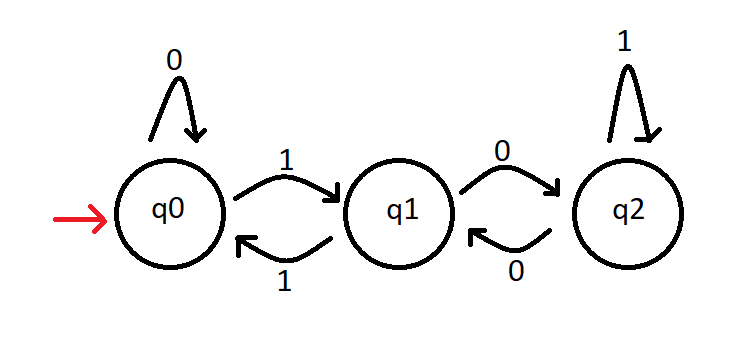
\includegraphics{01.png}

\underline{Доказано}

\subsection{Задача 6}

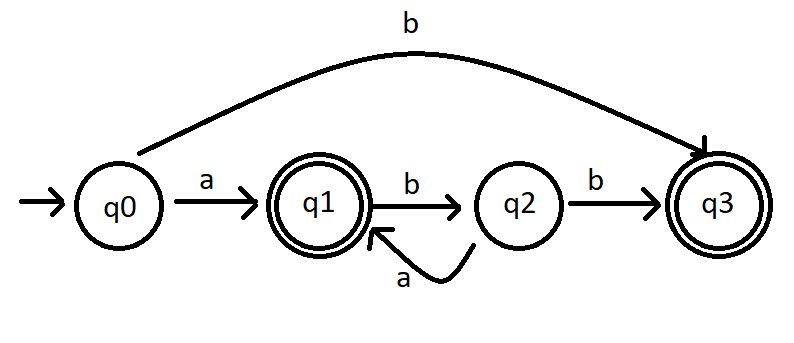
\includegraphics[scale=0.7]{05.png}

Построим табличку непринимающих состояний и принимающих состояний и выполним алгоритм.

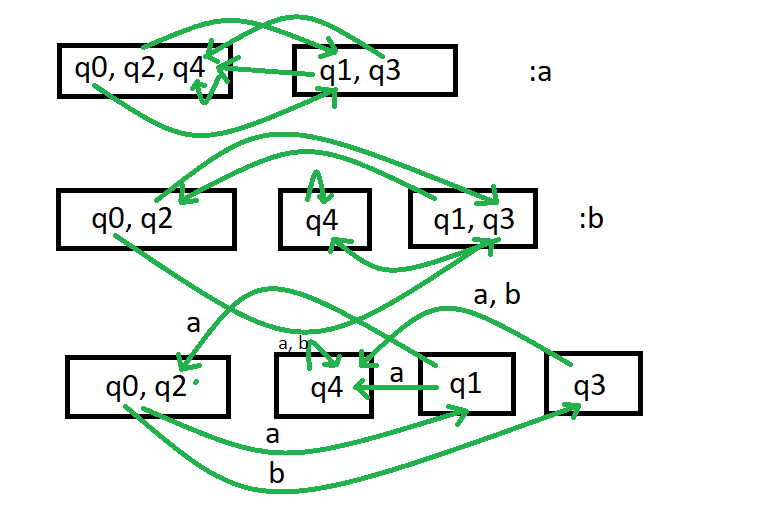
\includegraphics[scale=0.7]{03.png}

Ура, всё получилось, теперь можем построить ДКА из этой картинки.

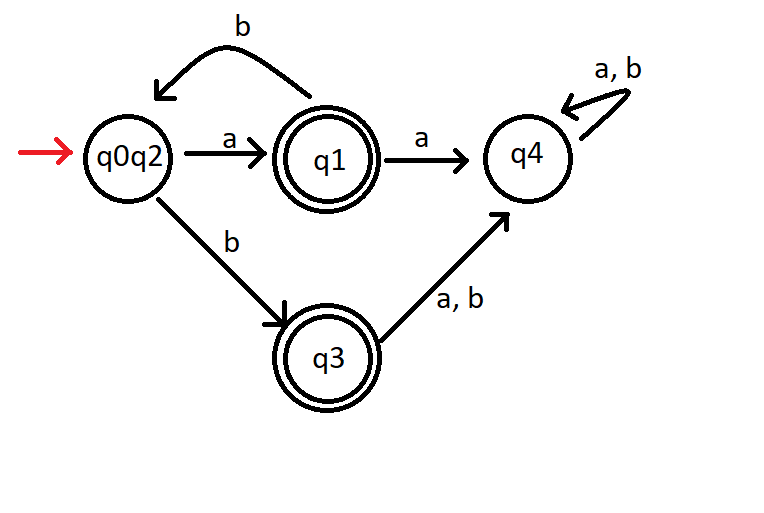
\includegraphics[scale=0.7]{04.png}

\subsection{ХУЙ}


\subsection{Задача 7}
L = \{a$b^{2^i}$ | i $\geqslant$ 0 \} $\cup$ \{$b^j$ | j $\geqslant$ 0\} $\cup$ \{$a^mb^n$ | m > 1, n $\geqslant$ 0 \}
\newline
$L_1$ = \{a$b^{2^i}$ | i $\geqslant$ 0 \}
\newline
$L_2$ = \{$b^j$ | j $\geqslant$ 0\} 
\newline
$L_3$ = \{$a^mb^n$ | m > 1, n $\geqslant$ 0 \}
\newline
L = $L_1 \cup L_2 \cup L_3$

Теперь, докажем, что лемма о накачке выполняется для этого языка L.

Рассмотрим лемму: для $L_1$ можем взять $p_1 = 1$, $x = \epsilon$, y = a(|y| = 1 $\leqslant$ $p_1$),
z = $b^{2^i}$. Тогда при k = 0 $xy^kz = b^{2^i} \in L_2 \subseteq L;$
При k = 1 $xy^kz = ab^{2^i} \in L_1 \subseteq L$.
При k > 1 $xy^j = a^jb^{2^i} \in L_3 \subseteq L$. Значит все слова из $L_1$ удовлетворяют лемме о накачке для L.

Рассмотрим лемму: для $L_2$ можем взять $p_2 = 1$, $x = \epsilon$, y = b(|y| = 1 $\leqslant$ p), z = $b^{j-1}$.
Тогда $xy^kz = b^{j+k-1} \in L_2 \subseteq L$. Значит все слова из $L_2$ удовлетворяют лемме о накачке для L.

Для $L_3$ можно построить ДКА $\mathcal{A}_3$. Приведу его ниже:

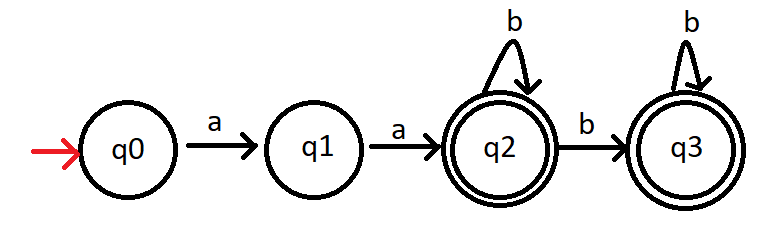
\includegraphics{02.png}

Значит для $L_3$ выполняется лемма о накачке: $\exists p_3 \forall \omega \in L_3 : |\omega| > p_3, \exists xyz = \omega$
$((y \neq \epsilon) \wedge (|xy| \geqslant p_L)) \wedge (\forall i \geqslant 0$ $xy^iz \in L))$ $\rightarrow$ $xy^iz \in L$.

\underline{Доказано}

Теперь докажем, что $L \notin REG$.
$L_1 \cap L_2 = \emptyset$, $L_1 \cap L_3 = \emptyset$, $L_2 \cap L_3 = \emptyset$.
$L1 = L \ (L_2 \cup L_3)$.
REG замкнуто относительно разности и объединения, тогда от противного предположим, что L $\in$ REG, т.к. $L_3 \in REG$ по доказанному выше, а $\{b\} \in REG$ 
$\rightarrow L_2 = \{b\}^* \in REG, то (L_2 \cup L_3) \in REG \rightarrow L_1 \in REG.$

Но $L_1 \notin REG$.
Для него не выполняется лемма о накачке, т.е. 

$\forall p \exists \omega \in L : |\omega| > p, \forall xyz = \omega ((y = \epsilon) \bigvee (|xy| > p) \bigvee (\exists \geqslant 0 : xy^tz \notin L)) $

Теперь попробуем показать это:
Если взять $x = \epsilon$, y = a$b^k$, то $xy^0z = b^{2^i - k} \notin L_1$, если взять y = $b^k$, то $xy^iz = ab^{2^i - k + tk} = ab^{2^i + (t-1)k}$.
Если бы $L_1 \in REG$, то $\forall k > 0$ $\forall t \geqslant 0$ $2^i + (t-1)k = 2^j$. Но при четном k, i > 0 или нечетного k, i = 0 это не будет выполнено ни для какого четного t, а в случае нечетного k, i > 0 или четного k, i = 0 - ни для какого четного t.

Следовательно лемма не выполнется, т.е. $L_1 \notin REG$ $\rightarrow$ $L \notin REG$

\underline{Доказано}




\end{document}